\chapter{Introducción}

%Análisis estadístico sobre números de teléfono en México, estadísticas sobre fraude que demuestren la veracidad de la problemática

% Se puede hablar también sobre lo necesario que es el uso de internet y redes sociales hoy dia

%Acceso a internet, uso de redes sociales, redes sociales laborales

%07-06-2025: todas las palabras que son anglisismos sin una traduccion directa deben ponerse en el glosario

El crecimiento exponencial en el uso de tecnologías móviles y plataformas de comunicación digital ha transformado la manera en que interactúan las personas. Según datos de la ENDUTIH 2023 \cite{UsoInternetPorEstado}, en México el 81.2\,\% de la población utiliza teléfono celular y el 96.1\,\% de los usuarios de internet en la Ciudad de México lo hace para comunicarse, principalmente a través de redes sociales y aplicaciones de mensajería. Esta adopción masiva ha traído consigo grandes beneficios, pero también ha abierto nuevas oportunidades para la comisión de delitos como el \textit{catfishing} y la extorsión digital.

La facilidad con la que se pueden crear perfiles falsos y establecer contacto anónimo en entornos digitales ha hecho que estos delitos proliferen, afectando especialmente a los jóvenes, quienes presentan la mayor penetración de internet (96.7\,\% en el grupo de 18 a 24 años). Además, cifras del INEGI (ENVIPE 2023) \cite{ENVIPE2023} reflejan un repunte en la tasa de incidencia de fraudes y extorsiones, situando a este fenómeno como una amenaza persistente en el ámbito digital.

El presente trabajo concentrara sus esfuerzos sobre las estafas catfishing y sextorsión puntualmente.

%2025-09-08 investigar si para esta parte Kaspersky o Norton tienen datos puntuales, un artículo habla sobre catfishing https://us.norton.com/blog/online-scams/what-is-catfishing?om_ext_cid=ext_social-_-Twitter-_-Educate-_-Video-_-Internet%20Security%20Center-_-kglobal

% COVID en pandemia: https://www.nbcnews.com/tech/tech-news/catfishing-during-coronavirus-how-old-internet-scam-still-tricks-people-n1197736

A lo largo del presente trabajo se encuentra una variedad de terminología de diferentes áreas del saber, se recomienda  consultar la sección glosario en la cual se definen todas aquellas palabras que a lo largo del trabajo estan escritas en itálica denotando ser un término presente en la sección antes mencionada.

\subsubsection{Personas usuarias de tecnologías de la información y comunicación}

\begin{figure}[H]
    \centering
    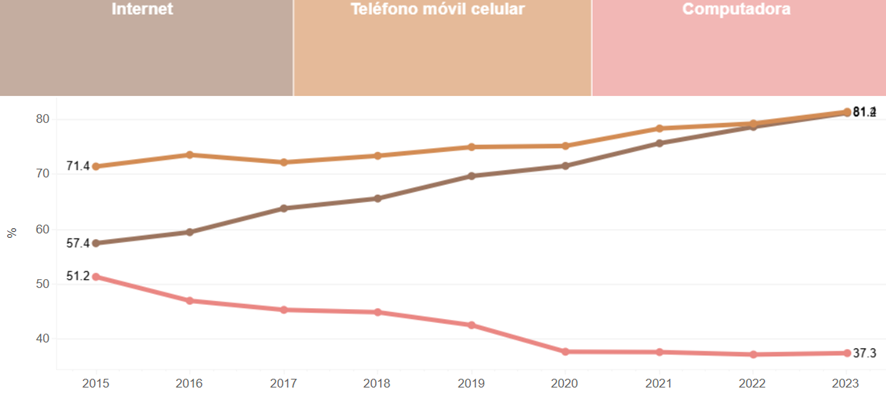
\includegraphics[width=1\linewidth]{imagenes/grafica1.png}
    \caption{orcentaje de usuarios de internet, telefonía móvil y computadora en México, 2023. Adaptado de Encuesta Nacional sobre Disponibilidad y Uso de Tecnologías de la Información en los Hogares (ENDUTIH)2023, por Instituto Nacional de Estadística y Geografía, 2024,\url{https://www.inegi.org.mx/programas/endutih/2023/\#informacion_general}.
    {\textcopyright} INEGI}
    \label{fig:1}
\end{figure}

\begin{figure}[H]
    \centering
    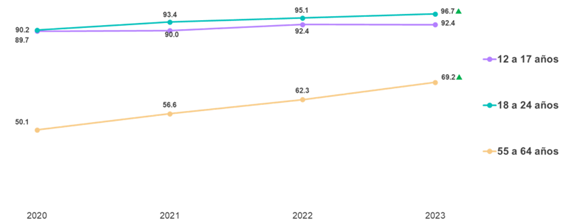
\includegraphics[width=1\linewidth]{imagenes/grafica2.png}
    \caption{Personas usuarias de internet según grupos de edad del 2020 al 2023\newline
    Acceso a internet por entidad federativa, 2023. Tomado de Encuesta Nacional sobre Disponibilidad y Uso de Tecnologías de la Información en los Hogares (ENDUTIH) 2023: Comunicado de prensa núm. 161/24, por Instituto Nacional de Estadística y Geografía, 2024, \url{https://www.inegi.org.mx/contenidos/saladeprensa/boletines/2024/ENDUTIH/ENDUTIH_23.pdf}. {\textcopyright} INEGI}
    \label{fig:2}
\end{figure}

Datos de la ENDUTIH 2024 muestran que los jóvenes de 18 a 24 años presentan la mayor penetración
de Internet en México (96.7 \%), lo cual coincide con su alta participación en redes sociales y aplicaciones de
citas. Esta combinación los convierte en un grupo con mayor exposición a estafas románticas y catfishing

\begin{figure}[H]
    \centering
    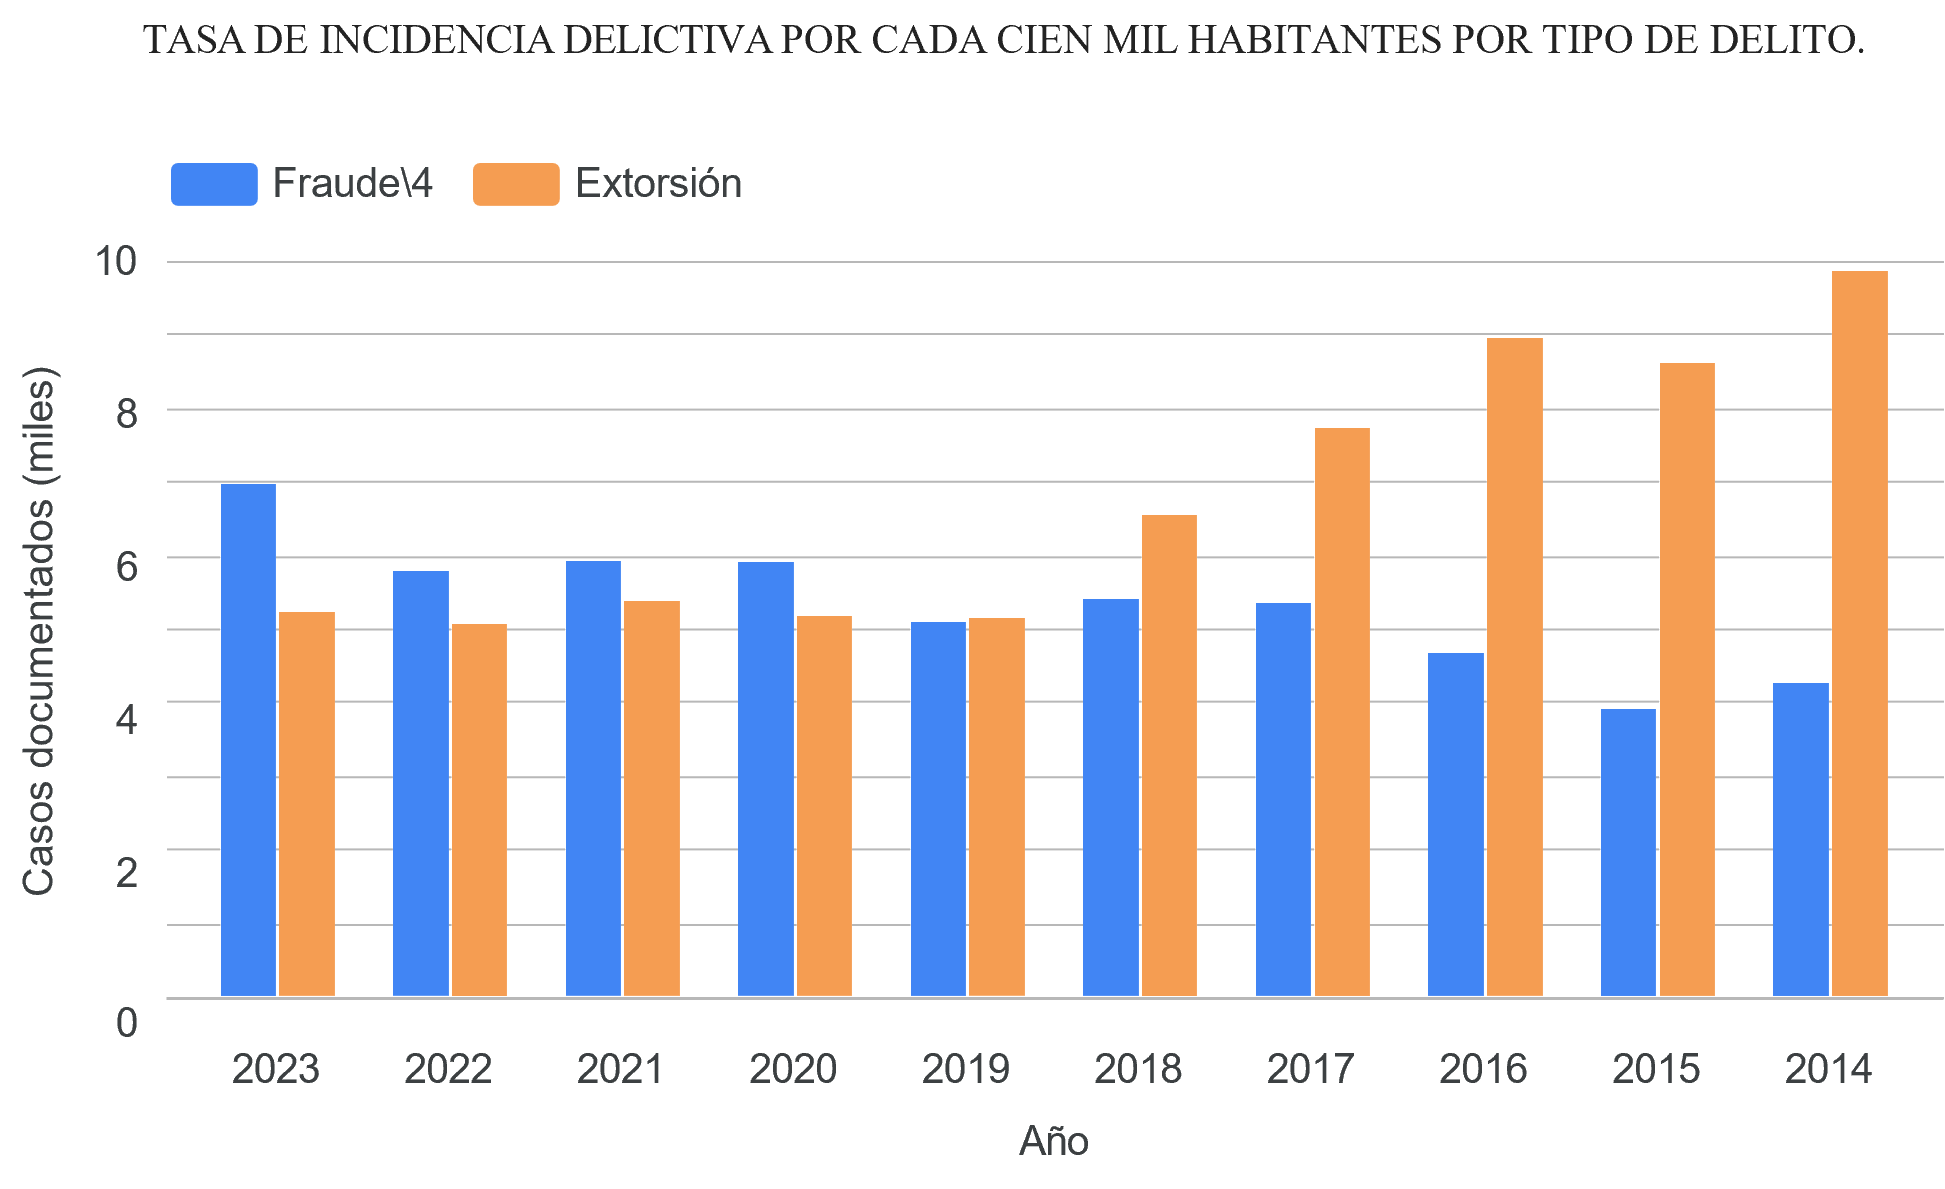
\includegraphics[width=1\linewidth]{imagenes/Tasa de incidencia delictiva por cada cien mil habitantes por tipo de delito..png}
    \caption{\cite{ENVIPE2023}}
    \label{fig:enter-label}
\end{figure}

\subsubsection{Servicios con los que cuenta la población}

Según la encuesta “Hogares con equipamiento de tecnología de información y comunicaciones, por entidad
federativa, según tipo de tecnología, 2023” en los hogares de la ciudad de México se cuentan con los servicios
de Internet 89.5 \%, telefonía 98.9 \%

\cite{ENDUTIH2023}

\subsubsection{Propósitos del uso de internet}

Según la base de datos “Usuarios de internet, por entidad federativa, según principales usos, 2023”, El
96,1 \% de los 7,897,062 de personas encuestadas en la ciudad de México , utilizan el ¿ para comunicarse, el
90,7 \% para redes sociales, el 37.7 \% para realizar operaciones bancarias, el 1.3 para pagos con tarjetas de
prepago.\cite{ENDUTIH2023}


\chapter{Problema y Objetivos}
 























\section{Descripción del problema}
Describir el problema de manera detallada, no definir la solución.



%%Planteamiento del problema


%Como este ahorita el planteamiento solo aborda el problema pero no como se piensa solucionar. En el planteamiento del problema se aborda primeramente el problema y posteriormente se puede hablar sobre los posibles enfoques con los que se podría solucionar el problema y dentro de estos enfoques

%Hablar sobre las consecuencias económicas, psicológicas, de privacidad

%24/05/2025: Vincular el catfishing con el crimen organizado en México (ej. "la matanza de cerdos" y asesinatos en call centers), Contactar con fiscalia para peticion de data set, añadir citas con BibTeX, Agregar matriz de confusión y investigar la evaluación de tiempo de inferencia para añadirlo al código de pruebas, descargar los papers para facilitarlos al asesor portillo en una carpeta

%07-06-2025: mas que el uso de internet "el uso de aparatos moviles en aspectos de vida cotidiana y la dependencia de estos"

%07-06-2025 00:52:55 : Mejorar la introducción del planteamiento del problema, enfocándose no solo en el crecimiento del internet, sino en el uso creciente de dispositivos móviles para resolver problemas cotidianos en ámbitos laborales, comerciales y personales (sentimentales)9.
Hoy en día el crecimiento de internet y aspectos multifactoriales han dado como producto un crecimiento de las estafas en línea y diversos tipos de extorción a través de las redes sociales, en la actualidad este tipo de fenómenos son principalmente efectuados dentro de los servicios de mensajería instantánea, los cuales se convierten en una oportunidad que tienen los
ciberdelincuentes para establecer contacto con diferentes usuarios a lo largo del mundo de manera anónima, la falta de
evidencia documentada sobre las estafas y casos de extorción en medios digitales también forma parte principal de los problemas en la agilización de los procesos que enfrentan las autoridades judiciales

video:
.......................................
En este video, El Heraldo de México expone informacion proporcionada por la policia cibernetica de la ciudad de Mexico con fin de divulgar los diversos riezgos que se corren al navegar en linea, se menciona que "los niños y adolescentes no tienen consienticacion sobre los peligros de compartir informacion en internet, en especial las fotografias de menores y las historias", aspecto altamente relacionado con diversos fraudes incluidos el catfishing y la sextorcion

% ESTA PARTE HABLA DE COMO LA POLICIA LIDIA CON EL PROBLEMA, DEBERIA IR EN LA PROBLEMATICA?

%formas en que la policia cibernetica aborda el problema
%* informando a la ciudaddania sobre
%* eortar a tener medidas de seguridad
%* involucrar a los padres en el seguimiento de actividades de sus hijos en linea, estableciendo horarios y limites de uso, hablar con los niños para enseñar a identificar contenido inapropiado, supervizar las apps de uso, mantener dialogo constante con los menores, uso de tecnologias de control parental para proteger la privacidad, fomentar la apertura comunicativa con hijos para llevar un caso asi a la denuncia

Finalmente el video tambien da un dato alarmante que esclarece la magnitud del problema que representan este tipo de fraudes dentro del pais pues se afirma que  "Mexico supera la media global en ciberataques, el 48\% reporta ataques a sus telefonos moviles" este dato en particular otorga la prespectiva que la mayoria de fraudes en linea se efectuan dentro de telefonia movil en redes sociales y comunmente dentro de mensajeria instantanea
\cite{heraldo1youtube}

los adultos mayores son frecuentemente víctimas de los ciberdelincuentes por su falta de familiaridad con la tecnología, y a que al no haber crecido en un entorno tecnológico son más susceptibles a las trampas que emplean técnicas de ingeniería social

%07-06-2025: los numeros del 35 y 26 porciento deberia sumar 100%, en cullo caso acompletar con "otros"
las plataformas más utilizadas para realizar este tipo de prácticas son las de mensajería instantánea en un 35 por ciento, llamadas y mensajes de texto con 26 por ciento

los especialistas de la Policía Cibernética mencionan que  Si alguien que conoció por internet declara su amor en poco tiempo y luego solicita dinero, es muy probable que sea una estafa. No enviar dinero ni compartir información personal con gente que no conozca físicamente.
%07-06-2025: en las estafas inicialmente no suele comienzar con dinero, pueden ser recargas o factores multiples, considerarlo para nota aclaratoria

%07-06-2025: las citas deben de ponerse inmediatamente

\cite{heraldo2025ciberdelitos}

Las estafas como el catfishing y la sextorcion no son una circunstancia trivial pues estos no solo son casos efectuados por grupos cibercriminales que operan por voluntad propia, este fenomeno lamentablemente es parte de un problema mucho mayor que se afronta en Mexico,  el crimen organizado.

Un ejemplo puntual de lo anterior mencionado es el caso de Andrea y Federico, un noviazgo que fue separado tras que Federico acudiera a una supuesta oferta de trabajo que "No exigía experiencia, tampoco un largo proceso de selección. Contratación inmediata", el dia siguiente 9 de diciembre, Federico envio un ultimo mensaje a su pareja Andrea, posterior a esto no se le volvio a ver, "El chico, de 23 años, se había esfumado".

este caso forma parte de un fenomeno criminal de escala mundial, nombrado por la interpol como "pic butchering", "matanza de cerdos" por los cuerpos policiacos en México

Dada la magnitud del fenomeno en marzo del 2024 la Interpol envio un mensaje a 196 paises incluido México para alertar sobre el mismo.

En el contexto de México esta tendencia ha evolucionado al secuestro de personas como Federico para obligarlas a laborar en negocios con fachada de call centers dedicados a la estafa, ofertas falsas de empleo, protección a personas que ingresan por primera vez a una cárcel o un anexo o, incluso, a reclutamiento del crimen mediante videojuegos.

Pero por sobre todas las actividades este movimiento desde sus origenes en ASIA fue reconocido por obligar a los secuestrados a establecer vinculos amorosos con victimas para estafar economicamente a cambio de su libertad, cabe mencionar que en el contexto Mexicano se afirma que el dinero obtenido de estas estafas resultan en financiamiento para el mismo CJNG que gestiona estas actividades
%continuar redaccion de la nota
\cite{milenio2024cjng}


\section{Objetivo general}
Presentar el objetivo general, debe coincidir con el título del proyecto.


Diseñar un sistema de filtrado de mensajería instantánea para detección de las estafas catfishing y sextorsión mediante el refinamiento de un modelo largo de lenguaje delimitado al geolecto del español de la Ciudad de México.
%El "refinamiento" de los Modelos de Lenguaje a Gran Escala (LLM, por sus siglas en inglés, Large Language Models) se refiere al proceso de adaptar o mejorar un modelo previamente entrenado para tareas o dominios específicos, o para corregir comportamientos no deseados.

%Es importante distinguirlo del "preentrenamiento" inicial, donde el LLM aprende las bases del lenguaje a partir de una vasta cantidad de datos. El refinamiento toma ese modelo base y lo ajusta para un uso más preciso y contextualizado.

%28-06-2025: con repecto al problema del enmascaramiento de palabras "ej algoritmo de youtube": en las estructuras de software, existe el mantenimiento como tarea, en ese caso puede darse la actualizacion de terminologia o de cambio de modelos con nuevos emergentes





\subsection{Objetivos específicos}

% Considerar lo siguiente para la redaccion de objetivos especificos: Seleccionar un modelo de lenguaje base adecuado balanceando tamaño y habilidad para identificación de
catphising y extorción mediante la ejecución de pruebas en el entorno de jypiter lab

Implementar diferentes pruebas para analizar el desempeño de diferentes modelos de lenguaje en la clasificacion de catfishing y sextorcion y con los datos fundamentar la existencia de un modelo largo de lenguaje igual o menor a 8b que pueda detectar efectivamente las estafas o de caso contrario optar por un enfoque basado en el fine tuning de uno de los modelos con mejores metricas  

La restricción de emplear estrictamente un modelo menor a 8b surge por el requerimiento de tiempo de respuesta cercano al tiempo real propio de la naturaleza y definición del proyecto el cual tiene por objetivo alertar al usuario con notificaciones antes de ser victima del fraude

El otro requerimiento esta fundamentado en los limites y alcances de esta investigacion para la cual no se contempla un presupuesto destinado a la compra de tiempo de computacion o hardware con prestaciones que permitan la ejecucion de modelos con mayor cantidad de parametros

Entorno de las pruebas
* Las pruebas se realizaron en un entorno de jypiter 

El proyecto plantea iniciar a partir de un modelo largo de lenguaje ya entrenado y funcional para ello se plantea una revision y posterior evaluacion de los modelos de lenguaje mas populares que posean una version ¿cuantizada? para ejecucion local en equipos de baja prestacion con una sola GPU,

Para la seleccion del modelo de lenguaje base se requiere conocer el desempeño que poseen los diferentes modelos al momento de identificar los fenomenos de catfishing y sextorcion.

Para esta primer evaluacion se consideraran 3 enfoques diferentes

%%%%%%%%%%%%%%%%%%%%%%%%%%%%%%%%%%%%%%%%%%%%%%%%%%%%%%%%%%%%%%%%


Listar los objetivos específicos, todos aquellos necesarios para llegar al objetivo general.



%Simplificar la redacción de los objetivos priorizando los action verbs, ya en el marco teorico se puede hablar mas detenidamente sobre las características profundoas de los modelos y todo lo contemplado en profundidad tecnica Simplificar la redacción de los objetivos priorizando los action verbs, ya en el marco teorico se puede hablar mas detenidamente sobre las características profundoas de los modelos y todo lo contemplado en profundidad tecnica

%metodologicamente siendo purista se requiere que cada objetivo tenga solo un verbo,

\begin{itemize}
    \item Investigar el estado del arte actual de los modelos largos de lenguaje
    %caracteristicas llms,
    \item Generación de datos sintéticos puntualmente mensajes maliciosos categorizados como catphishing y sextorcion mediante uso de modelos largos de lenguaje
    %con respecto a este de generacion, hablar de la necesidad el por que se hara sintetica,ente, esta justificacion va en marco teorico y hablar de como se realizo la base de datos esto ira en desarrollo
    %en marco teorico tambien hablar de como es el proceso de entrenamiento en un llm
    %transfor learning = fine tuning

    \item Recolección de datos reales sobre mensajes fraudulentos categorizados como catfishing y sextorción.

    \item Evaluar el desempeño de varios modelos en la identificación de catfishing y sextorsión utilizando refinamiento a traves de estrategias de prompting (zero-shot y few-shot).
   
    \item Planificar un enfoque de pruebas de desempeño basado en entrenamiento con ajuste fino en el supuesto de un desempeño deficiente con el enfoque en prompting

    %28-06-2025: Esta bien pero puede que se modifique mas adelante segun sea el resultado de las pruebas

    \item Desarrollar una aplicacion web de mensajeria instantanea a manera de interfaz de usuario para montarlo como entorno de produccion
    %07-06-2025: este objetivo se mencionara en justificacion y desarrollo, hay comentarios relacionados con esta fecha en dichas secciones

    %28-06-2025: Investigar los metodos de cobro por unidad de medicion como lo son, por tiempo de uso, por memoria, por volumen de peticiones, por numero de consultas, por usuarios conectados, por datos transmitidos, etc, entonces depende de AWS es de los mas economicos con planes para alumnos, investigar tambien las herramientas a ocupar si VM, u otros elementos, portillo dice que se puede tener un modelo y se dan un volumen de peticiones como 500 peticiones y con el plan institucional incluso no se paga
   
    %28-06-2025: escalamiento, y promociones de escalamiento, son formas de mejorar o crecer la solucion como el vertical y horizontal que ofertan los IaaS, portillo no recomenda meterse en eso actualmente, podria ser a posterior,

\end{itemize}

%Como el tecnisismo prompt puede tener colision en el contexto de las CLIs, investigar como poner notas al pie de pagina para distinguir a que se refiere en nuestro ámbito o directamente aconsejar visitar la sección de glosario de términos, analizar esto no solo para prompt sino para tantos se requieran (conviene mejor una redaccion glocal que recomiende visitar el glosario)

Seguir uno de los dos enfoques para llevar a cabo el fine tuning en medida de haber conseguido resultados de identificaci{\'{o}}n solidos con el modelo seleccionado y el conjunto de prompts refinados

%La selección de Android debe ser justificada también, puede ser en marco teorico o en el desarrollo, en dhica parte habría que resaltar las ventajas y desventajas de cada tecnología para justificar la elección de la misma, se puede considerar la experiencia de los autores con la tecnología pero es mejor desde las características técnicas y de servicio como los que incluyen soporte técnico en contraste con el open sourse, un aspecto puede ser factor socioeconómico de México.

%Migrar el modelo refinado mediante fine tuning al ecosistema de Andoid mediante la tecnolog{\'{i}}a LiteRT para ejecutarlo como un servicio local en el dispositivo



\section{Límites y Alcances}
\subsection{Límites}
Listar los límites, que no se va a hacer.

\subsection{Alcances}
Listar los alcances, hasta donde se va a llegar.


%aplica para limites y alcances

%fuentes que lo sostienen: (REVISAR)
%Prompt de busqueda: ¿las estafas catfishing y sextorcion poseen una relación directa incluso de dependencia mutua en la mayoría de casos? responde con estudios en publicaciones oficiales, foros de ciberseguridad oficiales
%https://www.tandfonline.com/doi/full/10.1080/01639625.2024.2317904?utm_source=chatgpt.com#abstract
%https://www.sciencedirect.com/science/article/abs/pii/S0747563223004843?utm_source=chatgpt.com
%https://www.wired.com/story/child-sextorition-scam-compounds-southeast-asia/?utm_source=chatgpt.com





\section{Justificación del proyecto} 
¿Que problema resuelve este proyecto?, ¿para quien será de utilidad?, ¿quien se ve beneficiado?, ¿qué  ventajas tiene con respecto a otros proyectos parecidos?


%La justificación es puramente el por que se tiene que hacer, la parte de justificar las tecnologías e infraestructura esta mas de la mano del marco teorico o el desarrollo, la parte de la falta de evidencias también puede gihurar en la justificacion

%Altamente Relacionado con la hipótesis pues en la justificación se hablara de lo que beneficiaria el desarrollo de la solución planteada desde la hipotesis

%07-06-2025: se puede mencionar brevemente el aspecto de por que usar web app
